\section{整体设计}
\subsection{数据库设计}

本系统采用分层的数据架构设计,包括数据处理层和规范化数据层两个层次:
\begin{enumerate}
  \item 数据处理层
  \begin{itemize}
    \item 目的:支持数据采集和清洗的ETL过程
    \item 特点:
    \begin{itemize}
      \item 保留原始数据格式,便于追溯和验证
      \item 允许数据冗余,不强制遵循3NF
      \item 支持增量更新和批量处理
    \end{itemize}
    \item 组成:
    \begin{itemize}
      \item 原始数据表:分别存储BOSS直聘和猎聘网的原始爬虫数据
      \item 暂存数据表:存储统一格式和质量检查后的中间数据
    \end{itemize}
  \end{itemize}

  \item 规范化数据层
  \begin{itemize}
    \item 目的:
    \begin{itemize}
      \item 提供高质量的规范化数据
      \item 支持复杂的数据查询和分析
      \item 保证数据一致性
    \end{itemize}
    \item 特点:
    \begin{itemize}
      \item 严格遵循3NF,消除数据冗余
      \item 建立完整的实体关系
      \item 支持事务处理
    \end{itemize}
    \item 组成:
    \begin{itemize}
      \item 基础实体表:包含用户、公司、职位、地址四个核心实体
      \item 关联关系表:维护实体间的多对多关系
      \item 物化视图:预计算常用查询结果,提升查询性能
    \end{itemize}
  \end{itemize}
\end{enumerate}

\begin{figure}[htbp]
  \centering
  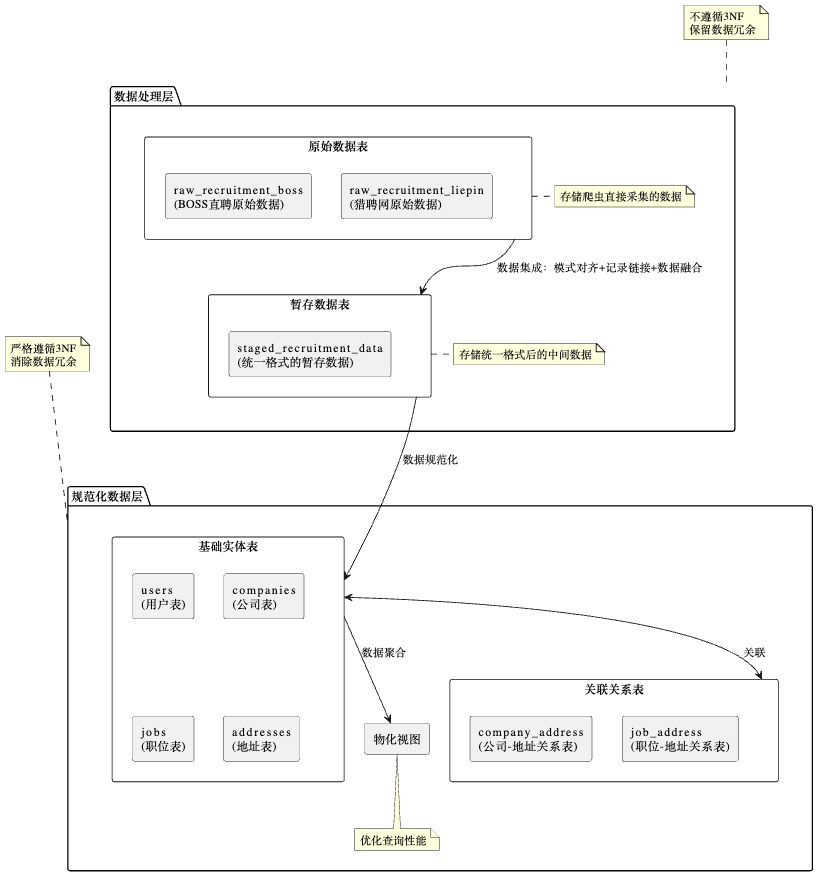
\includegraphics[width=0.8\textwidth]{figures/数据库概念设计.png}
  \caption{系统数据架构图}
  \label{fig:data_architecture}
\end{figure}


数据库采用分层架构设计,分为数据处理层和规范化数据层。这种分层设计有效分离了数据采集处理和业务数据存储的职责,使系统具有更好的可维护性和扩展性。

\subsubsection{数据处理层}
数据处理层不严格遵循第三范式,保留适度的数据冗余以支持数据处理和追溯。该层包含原始数据表和暂存数据表两类重要组件。原始数据表分别存储来自BOSS直聘和猎聘网的爬虫采集数据,完整保留了JSON格式的原始数据,并通过processed字段标记处理状态,支持数据的增量处理和历史追溯。

暂存数据表则作为数据集成的中间层,承担着数据规范化的重要职责。它通过统一的字段命名和格式规范,实现了不同来源数据的模式对齐。同时,暂存表还包含了一系列特殊设计字段,如record\_hash\_for\_linkage和duplicate\_group\_id用于数据去重,is\_master\_record和linked\_record\_ids用于关联记录管理,这些设计为后续的记录链接和数据融合提供了基础支持。

数据处理层的实体之间形成了清晰的数据流转路径:

\begin{itemize}
    \item 数据采集阶段:
    \begin{itemize}
        \item 爬虫程序分别从BOSS直聘和猎聘网采集数据
        \item 原始数据分别存入对应的原始数据表
        \item 通过processed字段标记数据的处理状态
    \end{itemize}
    
    \item 数据清洗阶段:
    \begin{itemize}
        \item 原始数据经过清洗后存入暂存数据表
        \item 统一数据格式,规范字段命名
        \item 进行数据去重和关联处理
    \end{itemize}
    
    \item 数据转换阶段:
    \begin{itemize}
        \item 暂存数据经过规范化处理
        \item 通过record\_hash\_for\_linkage进行重复检查
        \item 使用duplicate\_group\_id管理重复记录组
        \item 通过is\_master\_record标记主记录
    \end{itemize}
\end{itemize}

这种分层的数据处理设计确保了数据的可追溯性和处理过程的可控性,同时通过合理的字段设计,保证了数据处理的效率和准确性。

\subsubsection{规范化数据层}
规范化数据层严格遵循第三范式设计原则,通过消除数据冗余来保证数据一致性。该层主要由基础实体表、关联关系表和物化视图三部分构成。基础实体表包括用户、公司、职位和地址四个核心实体,每个实体表都独立管理其特有属性。关联关系表(company\_address和job\_address)则专门处理实体间的多对多关系,通过外键约束确保数据完整性。

为了平衡规范化设计带来的查询性能影响,该层还包含了物化视图组件。物化视图通过预先计算和存储常用查询结果,在保证数据一致性的同时提供了优秀的查询性能。这种设计既保持了规范化的优势,又解决了实际应用中的性能需求。

两个数据层之间通过明确的数据流向连接:原始数据经过清洗和转换进入暂存表,再经过规范化处理后存入实体表和关系表,最后通过物化视图提供高效的数据服务。这种渐进式的数据处理流程,确保了数据质量的同时,也保证了整个过程的可控性和可追溯性。

如图\ref{fig:data_architecture}所示,系统采用分层架构设计,将数据处理层和规范化数据层进行清晰分离。数据处理层包含BOSS直聘(raw\_recruitment\_boss)和猎聘网(raw\_recruitment\_liepin)的原始数据表,以及用于存储统一格式数据的暂存表(staged\_recruitment\_data),不严格遵循第三范式以支持数据处理和追溯。规范化数据层则严格遵循3NF范式,由用户(users)、公司(companies)、职位(jobs)、地址(addresses)四个基础实体表,以及公司-地址(company\_address)、职位-地址(job\_address)两个关联关系表组成,并通过物化视图(recruitment\_mv)优化查询性能。数据流向是从原始数据经过清洗后存入暂存表,再经规范化处理后存入实体表和关系表,最后通过物化视图提供高效的数据查询服务。


\subsection{后端设计}

在设计本系统时,面临着多个关键挑战:首先是需要处理来自不同招聘网站的异构数据,这些数据格式和结构各不相同;其次是需要确保数据的实时性和准确性,因为招聘信息经常会发生变化;最后是需要提供高效的数据查询和分析功能,以支持各种数据可视化和统计分析需求。

为了应对这些挑战,采用了分层架构设计,通过清晰的数据流向和模块划分,实现了从数据采集到数据展示的完整流程。如图\ref{fig:system_dataflow_simplified}所示,系统主要包含六个核心层次:外部数据源层、ETL处理层、数据存储层、CRUD层、API服务层和后台服务层。这种分层设计不仅使系统结构清晰,便于维护和扩展,还能够有效地隔离不同功能模块,提高系统的可靠性和可维护性。

\begin{figure}[htbp]
    \centering
    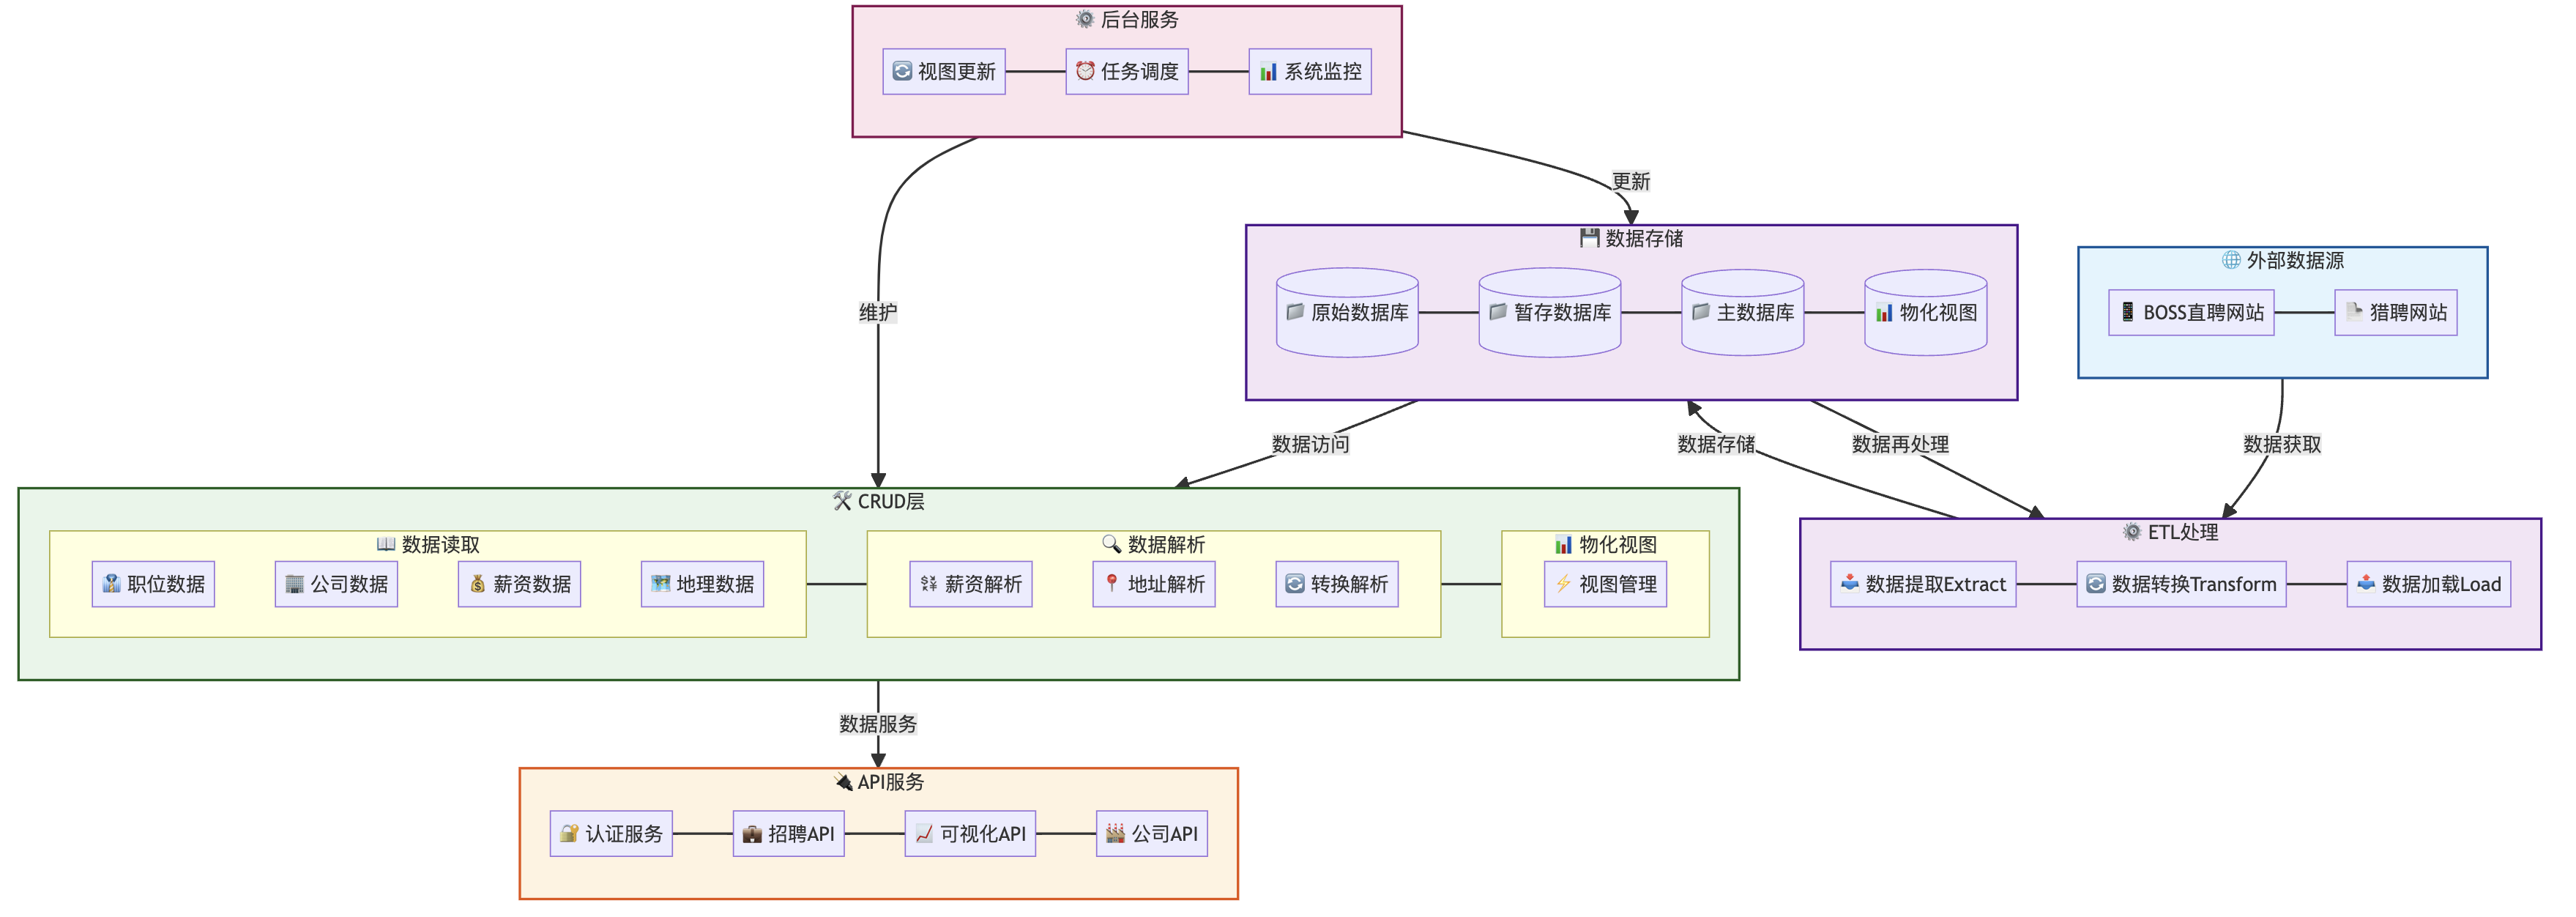
\includegraphics[width=1.0\textwidth]{figures/系统数据流图简化版.png}
    \caption{系统数据流图简化版}
    \label{fig:system_dataflow_simplified}
\end{figure}



图\ref{fig:system_dataflow}是系统数据流图的详细版本,展示了系统从数据采集到数据展示的完整流程。该图通过流程图的形式详细展示了系统的数据流向:从BOSS直聘和猎聘网站的数据源开始,数据首先经过ETL处理层的提取、转换和加载三个阶段,然后依次存储在原始数据库、暂存数据库、主数据库和物化视图中。CRUD层负责数据的基础操作,包括职位、公司、薪资和地理数据的读取与解析,以及物化视图的管理。API服务层则提供了认证、招聘信息、可视化和公司信息等对外接口。整个系统由后台服务层的任务调度器进行统一调度,通过物化视图更新服务保持数据的实时性,并通过系统监控确保各个模块的正常运行。这种层次分明的架构设计不仅确保了数据处理的完整性和可靠性,也为系统的扩展和维护提供了便利。

\begin{figure}[htbp]
    \centering
    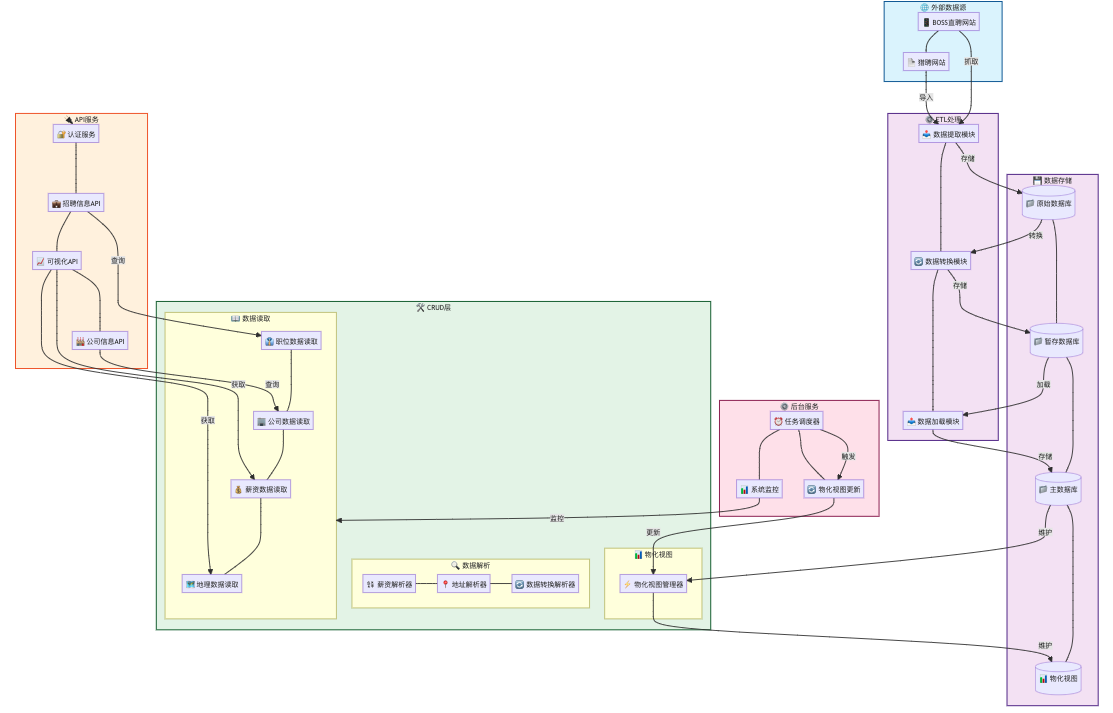
\includegraphics[width=1.0\textwidth]{figures/系统数据流图.png}
    \caption{系统数据流图}
    \label{fig:system_dataflow}
\end{figure}

\subsection{数据集成}
本系统实现了一个完整的ETL(Extract-Transform-Load)数据集成流程,将来自不同招聘网站的职位数据进行整合、清洗和标准化,最终加载到规范化的数据库中。整个过程包括数据抽取(Extract)、数据转换(Transform)和数据加载(Load)三个主要阶段。如图\ref{fig:ETL1}所示。

\begin{figure}[htbp]
    \centering
    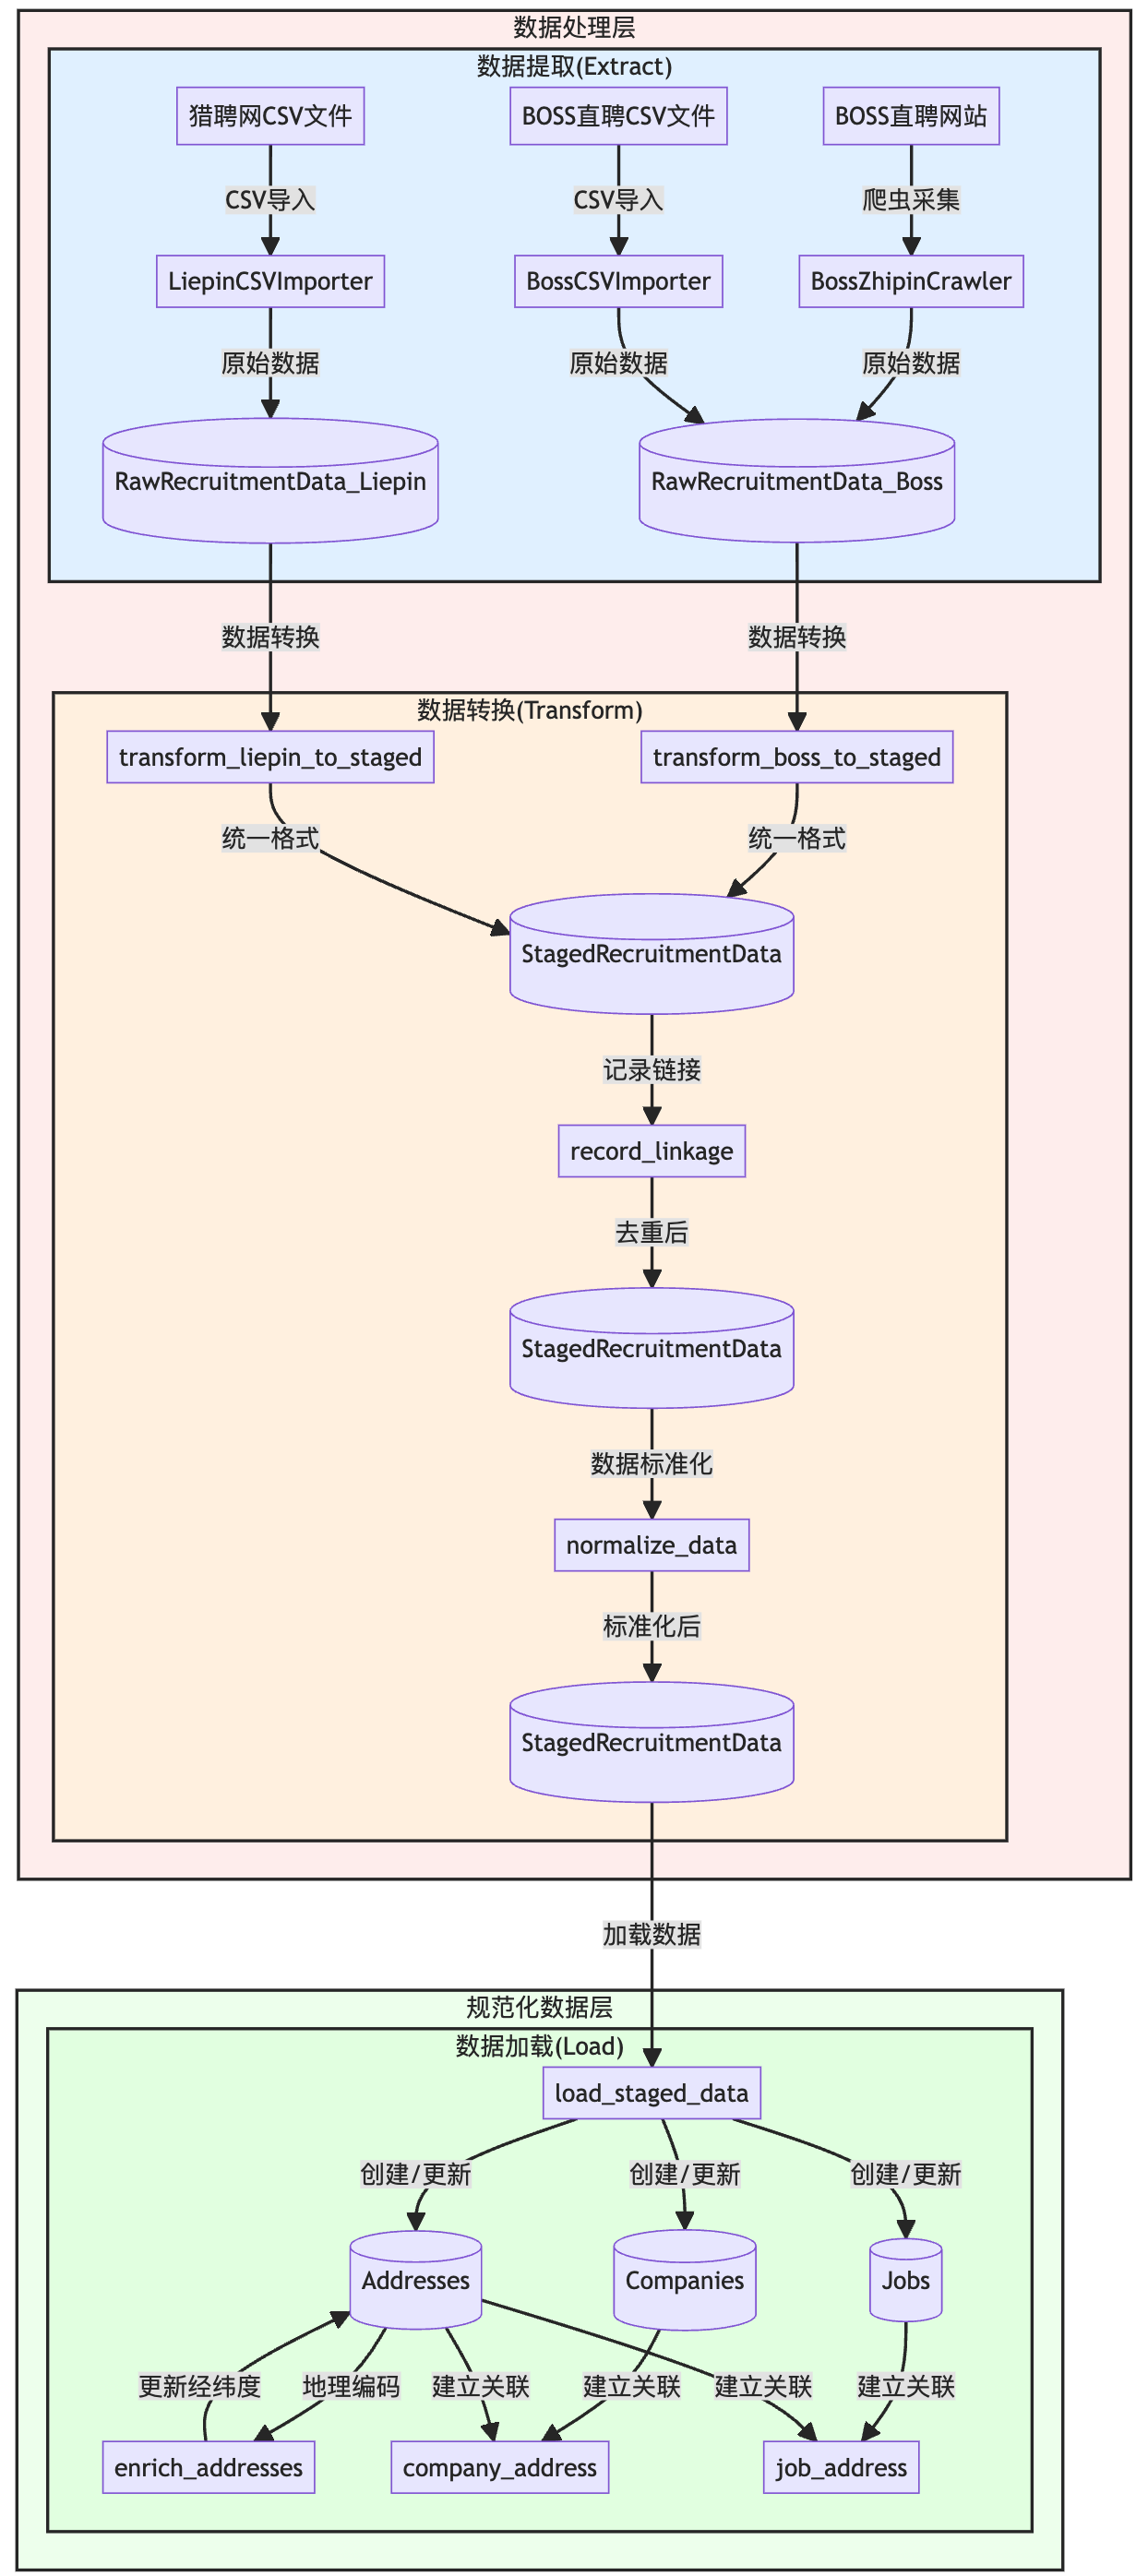
\includegraphics[width=0.6\textwidth]{figures/ETL.png}
    \caption{ETL数据集成流程}
    \label{fig:ETL1}
\end{figure}

\subsection{API实现}

系统的API层采用FastAPI框架实现,遵循RESTful架构设计原则,提供了一系列标准化的HTTP接口。

\subsection{前端设计}
本项目的前端采用Next.js框架,使用React和NextUI来构建页面和组件,使用Tailwind CSS进行样式设计。
特别地,我们采用Next.js最新推出的文件路由系统,将文件组织结构自动映射到网页路由。

前端通过API来获取后端通过Plotly生成的网页元素,并将其进行渲染。